\subsection{Bus Isolation Module (BI)}

The Bus Isolation Module (BI) allows the slave to interconnect its GPIO pins with equivalent pins of the \mu M module.
These pins are not designed to support voltages > 0 when the microcontroller is powered off.
Since the slave microcontroller
is powered on only during the transmission phase, the pins configured for I2C would effectively be back-powered via
the internal ESD protection diodes.

\subsubsection*{Specification}

The switch must have the following characteristics:
\begin{itemize}
    \item low power: this excludes mechanical switches like reed relays
    \item bidirectional
    \item 3.3V logic compatible
\end{itemize}

\subsubsection*{Implementation}

\begin{table}[H]
    \centering
    \begin{threeparttable}[b]
        \begin{tabularx}{\linewidth}{ >
                    {\hsize=0.25\hsize}X >
                    {\hsize=0.75\hsize}X >
                    {\hsize=1.25\hsize}X >
                    {\hsize=0.75\hsize}X >
                    {\hsize=2.0\hsize}X
            }
            Id    & BOM item                       & Order Code      & FF       & Rationale \\
            \midrule
            $U_1$ & \cite{noauthor_ts5a23157_2004} & TPD3S014-Q1/176 & VSSOP/10 & low Ron   \\
        \end{tabularx}
    \end{threeparttable}
    \caption{BI - BOM}
\end{table}




\begin{table}[H]
    \centering
    \begin{threeparttable}[b]
        \begin{tabularx}{\linewidth}{ >{\hsize=.15\hsize}X >{\hsize=1.35\hsize}X >{\hsize=1.5\hsize}X }
            Id & Issue                                       & Potential solutions \\
            \midrule
            1  & $U_{1,2}$ can not be back-powered.\tnote{1} & TMUX1574RSVR (TI)   \\
        \end{tabularx}
        \begin{tablenotes}
            \item [1]   Usually, the slave is not powered on when the master is powered off because
            the load switch for the slave power supply requires a logic H from the master to be on.
            However, when flashing (programming) the slave, the master could be switched off and in this
            case the supply voltage of $U_{1,2}$ if \SI{0}{\volt}.
        \end{tablenotes}
    \end{threeparttable}
    \caption{\mu M - Issues}

\end{table}
\clearpage


\begin{figure}[h]
    \centering
    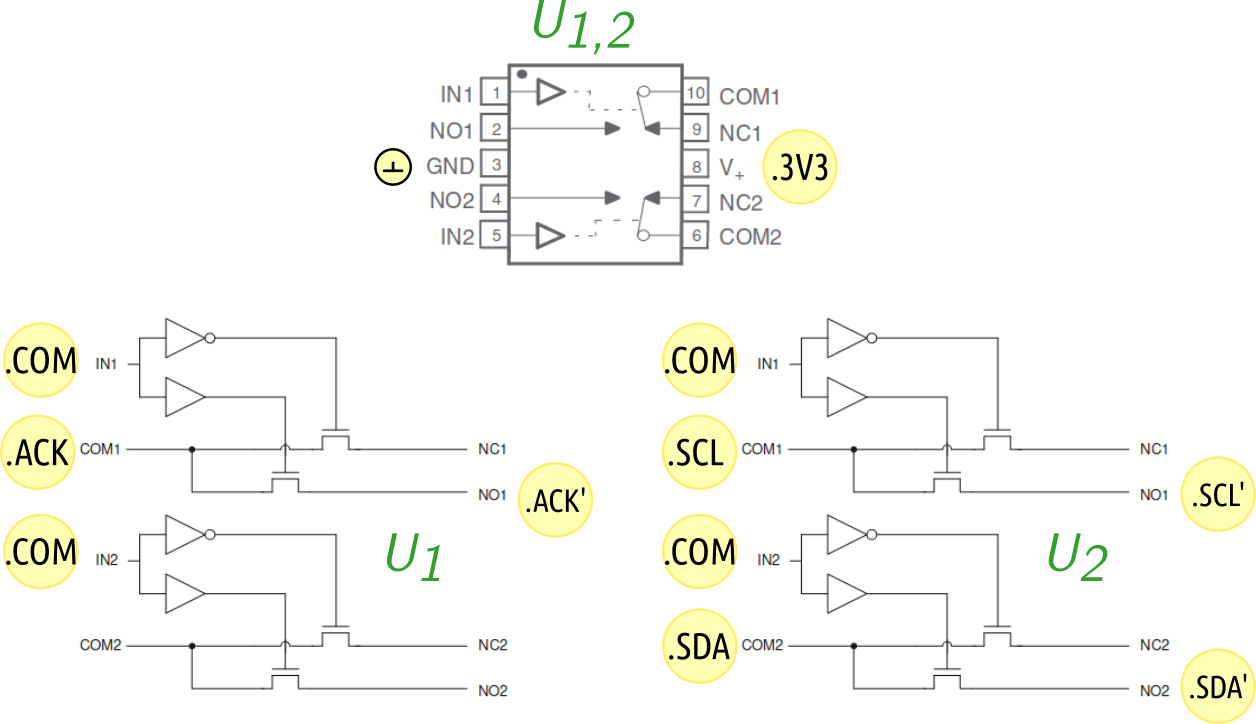
\includegraphics[width=1.0\textwidth]{MA/BI/BI}
    \caption{BI - schematic, based on datasheet \cite{noauthor_ts5a23157_2004}}
\end{figure}

\begin{table}[H]
    \centering
    \begin{threeparttable}[b]
        \begin{tabularx}{\linewidth}{ >
                    {\hsize=.25\hsize}X >
                    {\hsize=0.5\hsize}X >
                    {\hsize=.25\hsize}X  >
                    {\hsize=.5\hsize}X >
                    {\hsize=.25\hsize}X  >
                    {\hsize=3\hsize}X
            }
                  & \multicolumn{4}{c}{Pin mapping} &                                                                            \\
            \cmidrule(lr){3-6}
            Id    & Net                             & Nb. & Name          & Type            & Function                           \\
            \midrule
            $U_1$ & .COM                            & 1   & \texttt{IN1}  & \leftharpoonup  & switch 1 enable, driven by \mu S   \\
            $U_1$ & .ACK'                           & 2   & \texttt{NO1}  & \rightharpoonup & normally open, switch 1 output     \\
            $U_1$ & \Gnd                            & 3   & \texttt{GND}  & \Gnd            & \Gnd                               \\
            $U_1$ & .COM                            & 5   & \texttt{IN2}  & \leftharpoonup  & switch 2 enable, switch 2 not used \\
            $U_1$ & .3V3                            & 8   & \texttt{V+}   & \leftarrow      & power supply                       \\
            $U_1$ & .ACK                            & 10  & \texttt{COM1} & \leftharpoonup  & switch 1 input                     \\
            $U_2$ & .COM                            & 1   & \texttt{IN1}  & \leftharpoonup  & switch 1 enable, driven by \mu S   \\
            $U_2$ & .SCL'                           & 2   & \texttt{NO1}  & \rightharpoonup & normally open, switch 1 output     \\
            $U_2$ & \Gnd                            & 3   & \texttt{GND}  & \Gnd            & \Gnd                               \\
            $U_2$ & .SDA'                           & 4   & \texttt{NO2}  & \rightharpoonup & \Gnd                               \\
            $U_2$ & .COM                            & 5   & \texttt{IN2}  & \leftharpoonup  & switch 2 enable, switch 2 not used \\
            $U_2$ & .SDA                            & 6   & \texttt{COM2} & \leftharpoonup  & switch 2 enable, switch 2 not used \\
            $U_2$ & .3V3                            & 8   & \texttt{V+}   & \leftarrow      & power supply                       \\
            $U_2$ & .SCL                            & 10  & \texttt{COM1} & \leftharpoonup  & switch 1 input                     \\
        \end{tabularx}
        \begin{tablenotes}
            \item []
        \end{tablenotes}
    \end{threeparttable}

\end{table}
\clearpage


